\section{Introdução}


    Este trabalho apresenta um caso prático de sincronização de relógios usando o Network Time Protocol (NTP). O problema apresentado consiste em sincronizar as transições de estado de 2 semáforos de uma interseção sem que haja trocas de informações entre os eles. Deste modo, todos os semáforos irão utilizar um relógio abstrato, escravizado de acordo com um servidor NTP, para inferir o seu estado (Verde, Vermelho).
    
    Por exemplo, considerando a figura \ref{fig:diagramaEstrada}, quando o semáforo da via horizontal (1) está verde, o da via vertical (2) está vermelho. Ora, caso esta alteração de estado ocorra de $t$ em $t$ segundos, cada semáforo deve tomar essa decisão autonomamente de acordo com o seu relógio.
    Os dois relógios apresentam características diferentes, pelo que $t$ segundos no semáforo 1 pode representar $t + \delta$ segundos no relógio 2, pelo que a transição no 2 seria tomada $\delta$ segundos mais tarde. Normalmente, $\delta$ é um valor muito pequeno, pelo que quando considerando uma só transição este valor é irrelevante. Contudo, esta discrepância acumula com o tempo e, sem a aplicação de mecanismos de sincronização, pode levar ao caso de os dois semáforos estarem verdes ao mesmo tempo.
    Uma correta sincronização não irá colocar $\delta$ a zero, mas sim mantê-lo com um valor baixo o suficiente para que seja irrelevante para o sistema e constante ao longo do tempo. Para tal, cada semáforo irá atualizar periodicamente o "rate", o "offset" e o "delay" dos seus relógios com um servidor NTP, garantindo que $\delta$ não acumula infinitamente.  
    
    \begin{figure}[h]
        \centering
        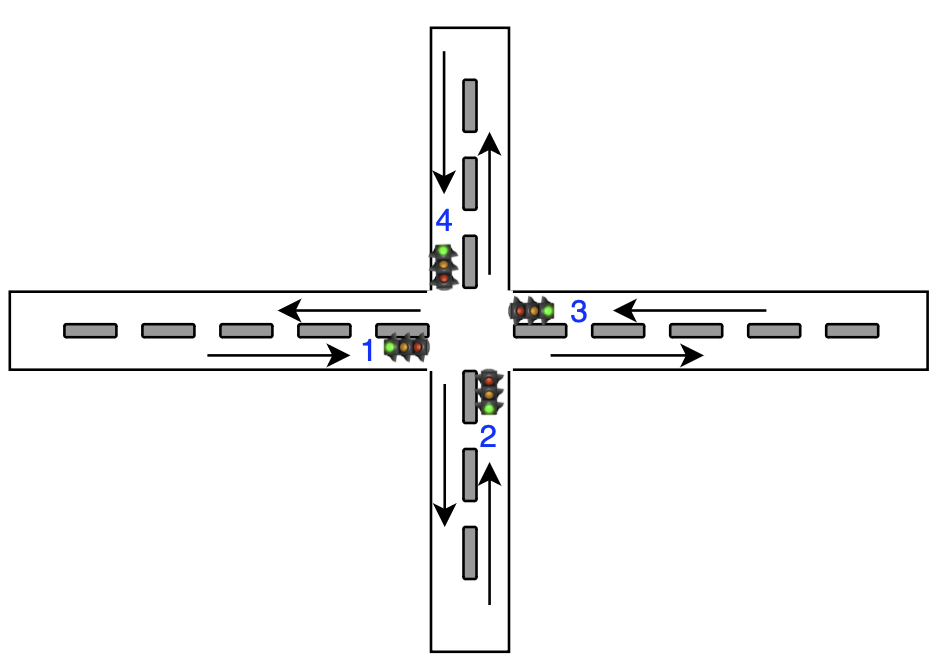
\includegraphics[width=0.8\linewidth]{figures/diagramaEstrada.png}
        \caption{Interseção de uma estrada}
        \label{fig:diagramaEstrada}
    \end{figure}

    Atualmente, as soluções para a mudança de estado dos semáforos pode ser agrupada em 2 grupos distintos, um primeiro baseado em sistemas de tempo fixo e um segundo em sistemas baseados em sensores. Para o primeiro caso, a mudança de estado é feita através de ciclos de tempo fixo, com base no relógio de cada semáforo. Contudo, maior parte dos semáforos não têm qualquer tipo de sincronização, tendo, em vez disso uma manutenção periódica aos seus relógios. O segundo caso utiliza sensores para medir o fluxo de trânsito, ou controlar a velocidade. Com base nos valores medidos por estes sensores, uma decisão é posteriormente tomada pelo sistema.
    
    